\documentclass[12pt,a4paper]{ctexart}
\usepackage[a4paper,margin=2.2cm]{geometry}
\usepackage{graphicx}
\usepackage{booktabs}
\usepackage{float}
\usepackage{enumitem}
\usepackage{array}
\usepackage{longtable}
\usepackage{amsmath}
\usepackage{caption}
\captionsetup{font=small}

\begin{document}

\begin{center}
{\LARGE \textbf{上机实验报告——特征选择数据集划分与线性回归}}\\[1em]
学号：1043220122 \hspace{2cm} 姓名：林鑫
\end{center}

\vspace{1em}

\section*{一、实验目的}
\begin{enumerate}[label=（\arabic*）]
\item 掌握特征选择的基本思路与实现方法，筛选有效特征。
\item 学会将数据集正确划分为训练集与测试集。
\item 掌握线性回归模型的构建、训练、预测与评价。
\item 巩固数据预处理流程。
\end{enumerate}

\section*{二、实验环境}
\begin{enumerate}[label=（\arabic*）]
\item 编程语言：Python
\item 核心库：
\end{enumerate}

\noindent pandas、numpy：数据读取与数值计算\\
\noindent sklearn：数据集划分、线性回归、评估指标\\
\noindent matplotlib/seaborn：可视化

\section*{三、实验数据介绍（对使用数据集作介绍）}
本实验所使用的数据集由 \texttt{get\_data.py} 抓取并导出，文件为 \texttt{code/沪深300\_最近三年.csv}。该数据集记录了沪深300指数近三年的日线交易数据，共有 725 条样本，包含 7 个原始字段，分别为：日期、收盘、开盘、高、低、交易量、涨跌幅。

本实验将“收盘价”作为回归模型的目标变量。其余字段中，“开盘价”“最高价”“最低价”“交易量”是主要候选特征；“涨跌幅”虽然也能反映价格变动情况，但它是由收盘价相对于前一日收盘价计算得到的，因此在建模时要特别考虑是否存在目标泄漏。由于数据本身带有明显时间顺序，因此在训练集和测试集划分时不能简单随机打乱，而应尽量保持时间先后关系。

\begin{table}[H]
\centering
\begin{tabular}{>{\raggedright\arraybackslash}p{3cm} >{\raggedright\arraybackslash}p{9.5cm}}
\toprule
字段 & 含义 \\
\midrule
日期 & 交易日期 \\
收盘 & 当日收盘价，作为目标变量 \\
开盘 & 当日开盘价 \\
高 & 当日最高价 \\
低 & 当日最低价 \\
交易量 & 当日交易量，原始格式带有 K \\
涨跌幅 & 相对前一交易日收盘价的涨跌百分比 \\
\bottomrule
\end{tabular}
\end{table}

为更直观地说明数据内容，表~\ref{tab:data-sample} 给出了数据集前 5 条记录示例。可以看出，原始数据已经按交易日组织完成，能够直接用于后续的数据预处理、特征筛选和线性回归建模。

\begin{table}[H]
\centering
\caption{沪深300近三年数据样例（前5条）}
\label{tab:data-sample}
\small
\begin{tabular}{c c c c c c c c}
\toprule
序号 & 日期 & 收盘 & 开盘 & 高 & 低 & 交易量 & 涨跌幅 \\
\midrule
0 & 2026-03-18 & 4,619.6200 & 4,648.7500 & 4,651.4300 & 4,604.5200 & 169361.41K & -0.38\% \\
1 & 2026-03-17 & 4,637.4400 & 4,685.5700 & 4,720.8600 & 4,637.3700 & 263021.91K & -0.73\% \\
2 & 2026-03-16 & 4,671.5600 & 4,669.2200 & 4,673.6900 & 4,621.8100 & 296215.07K & 0.05\% \\
3 & 2026-03-13 & 4,669.1400 & 4,669.0600 & 4,707.4200 & 4,659.5000 & 310772.01K & -0.39\% \\
4 & 2026-03-12 & 4,687.5600 & 4,700.7200 & 4,704.3800 & 4,654.3100 & 302986.82K & -0.36\% \\
\bottomrule
\end{tabular}
\end{table}

\section*{四、实验内容与步骤}

\subsection*{1. 数据加载与预处理（读取数据集,处理缺失值、异常值、重复行,分离特征矩阵和目标变量）}
首先读取原始 \texttt{CSV} 数据，并完成字段类型转换。具体来说，将日期字段转换为日期类型，便于后续按时间顺序排序和划分；将交易量中的 \texttt{K} 去除并转换为数值型；将涨跌幅中的百分号去除并转换为数值型。经过检查，原始数据中仅存在 1 个缺失值，位于涨跌幅字段，因此采用中位数填充。重复行数量为 0，说明原始数据整体较完整。

在异常值处理方面，本实验采用 IQR（四分位距）方法识别异常值，再使用截尾（clip）方式减弱极端值对模型训练的影响。识别结果显示：收盘价存在 6 个异常值，开盘价 3 个，最高价 1 个，最低价 2 个，交易量 24 个，涨跌幅 34 个。预处理完成后，除了从日期字段中构造年份、月份、日、星期等日历特征外，还进一步加入了更细化的特征工程：包括价格振幅（最高价减最低价）、开收盘价差、前 1/2/3 个交易日收盘价滞后特征、前 1 个交易日成交量滞后特征，以及基于历史收盘价构造的 3 日和 5 日滚动均值特征，同时补充成交量单日变化率。由于这些时序特征在序列起始位置会产生空值，因此删除了前 5 条无法完整构造特征的样本，最终剩余 720 条有效样本用于建模。

\begin{figure}[H]
\centering
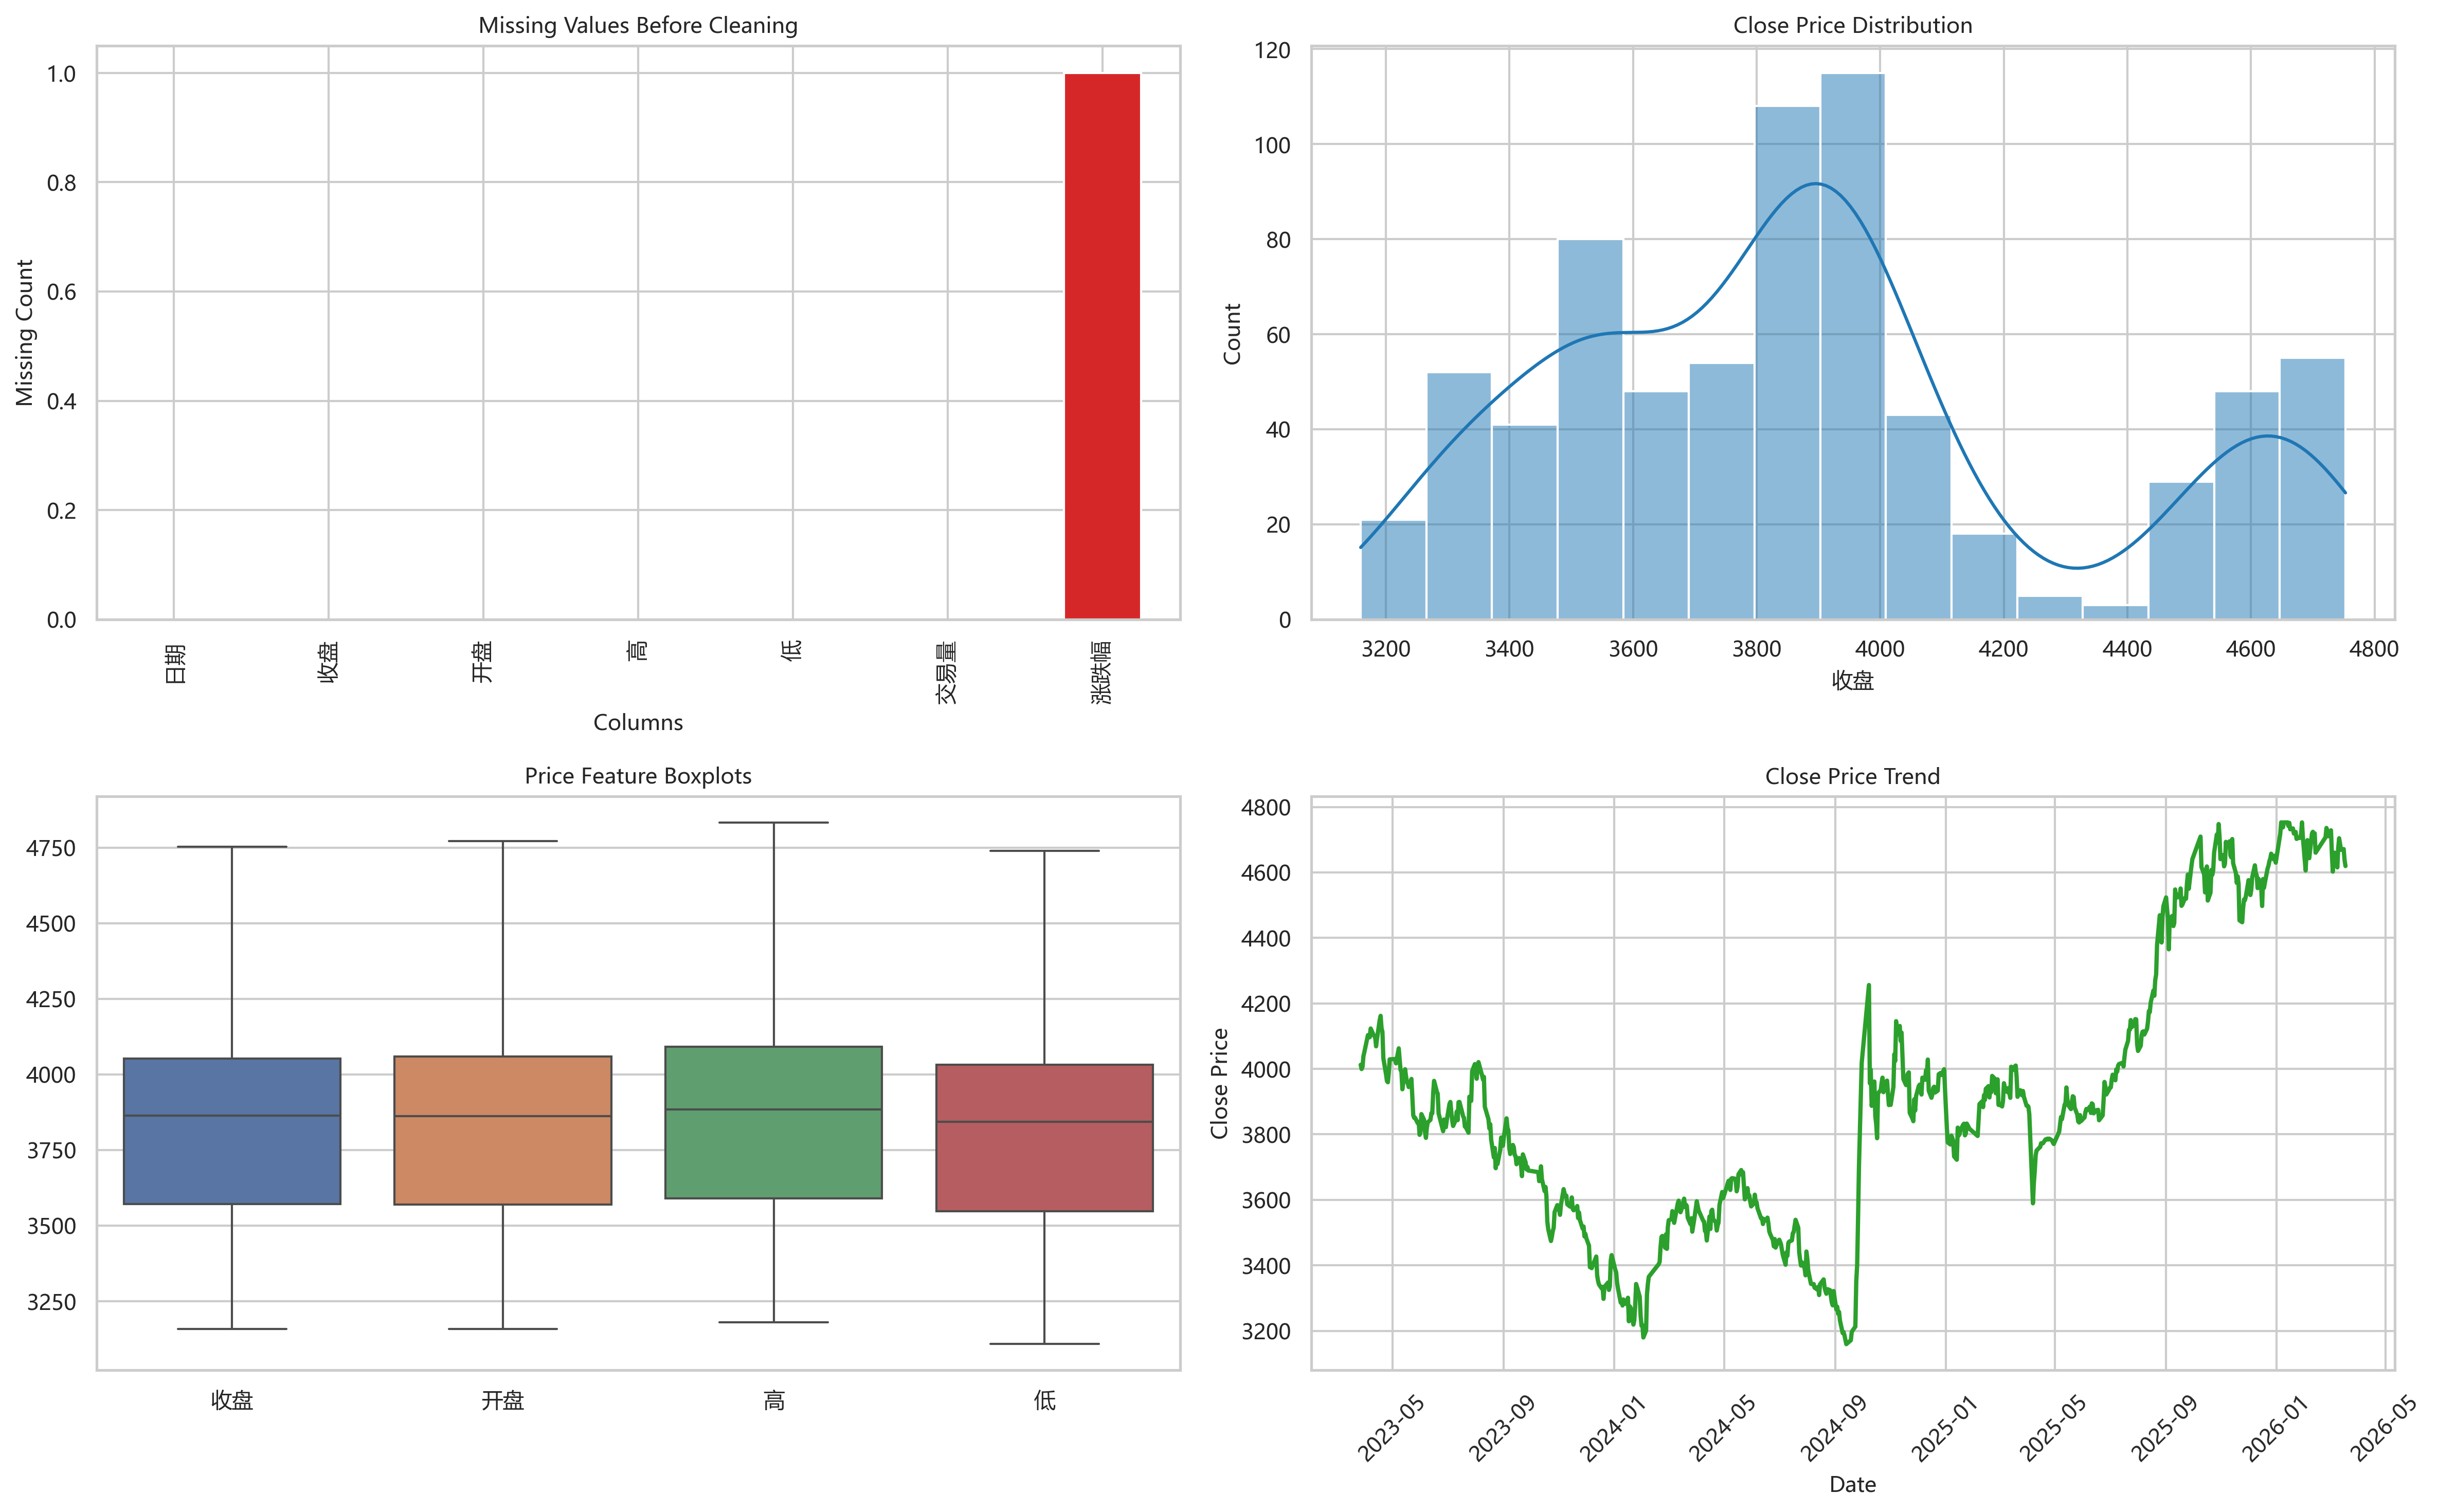
\includegraphics[width=0.92\textwidth]{../result/fig1_preprocess_overview.png}
\caption{数据预处理阶段的缺失值统计、收盘价分布、箱线图与走势}
\end{figure}

从图中可以看出，左上角缺失值柱状图表明只有“涨跌幅”字段存在 1 个缺失值，其余字段均完整，说明数据整体质量较高。右上角收盘价分布图显示样本主要集中在 3500 到 4100 区间，但在较高价格区间也有一部分样本，说明近三年指数水平存在明显阶段性变化。左下角箱线图说明价格类特征整体分布较集中，但在高位区域有少量离群点，这与 IQR 异常值检测结果一致。右下角收盘价走势曲线显示，沪深300指数在近三年内并非平稳波动，而是经历了先下降、后震荡、再明显回升的过程，说明时间因素对价格水平具有一定解释作用。

\begin{figure}[H]
\centering
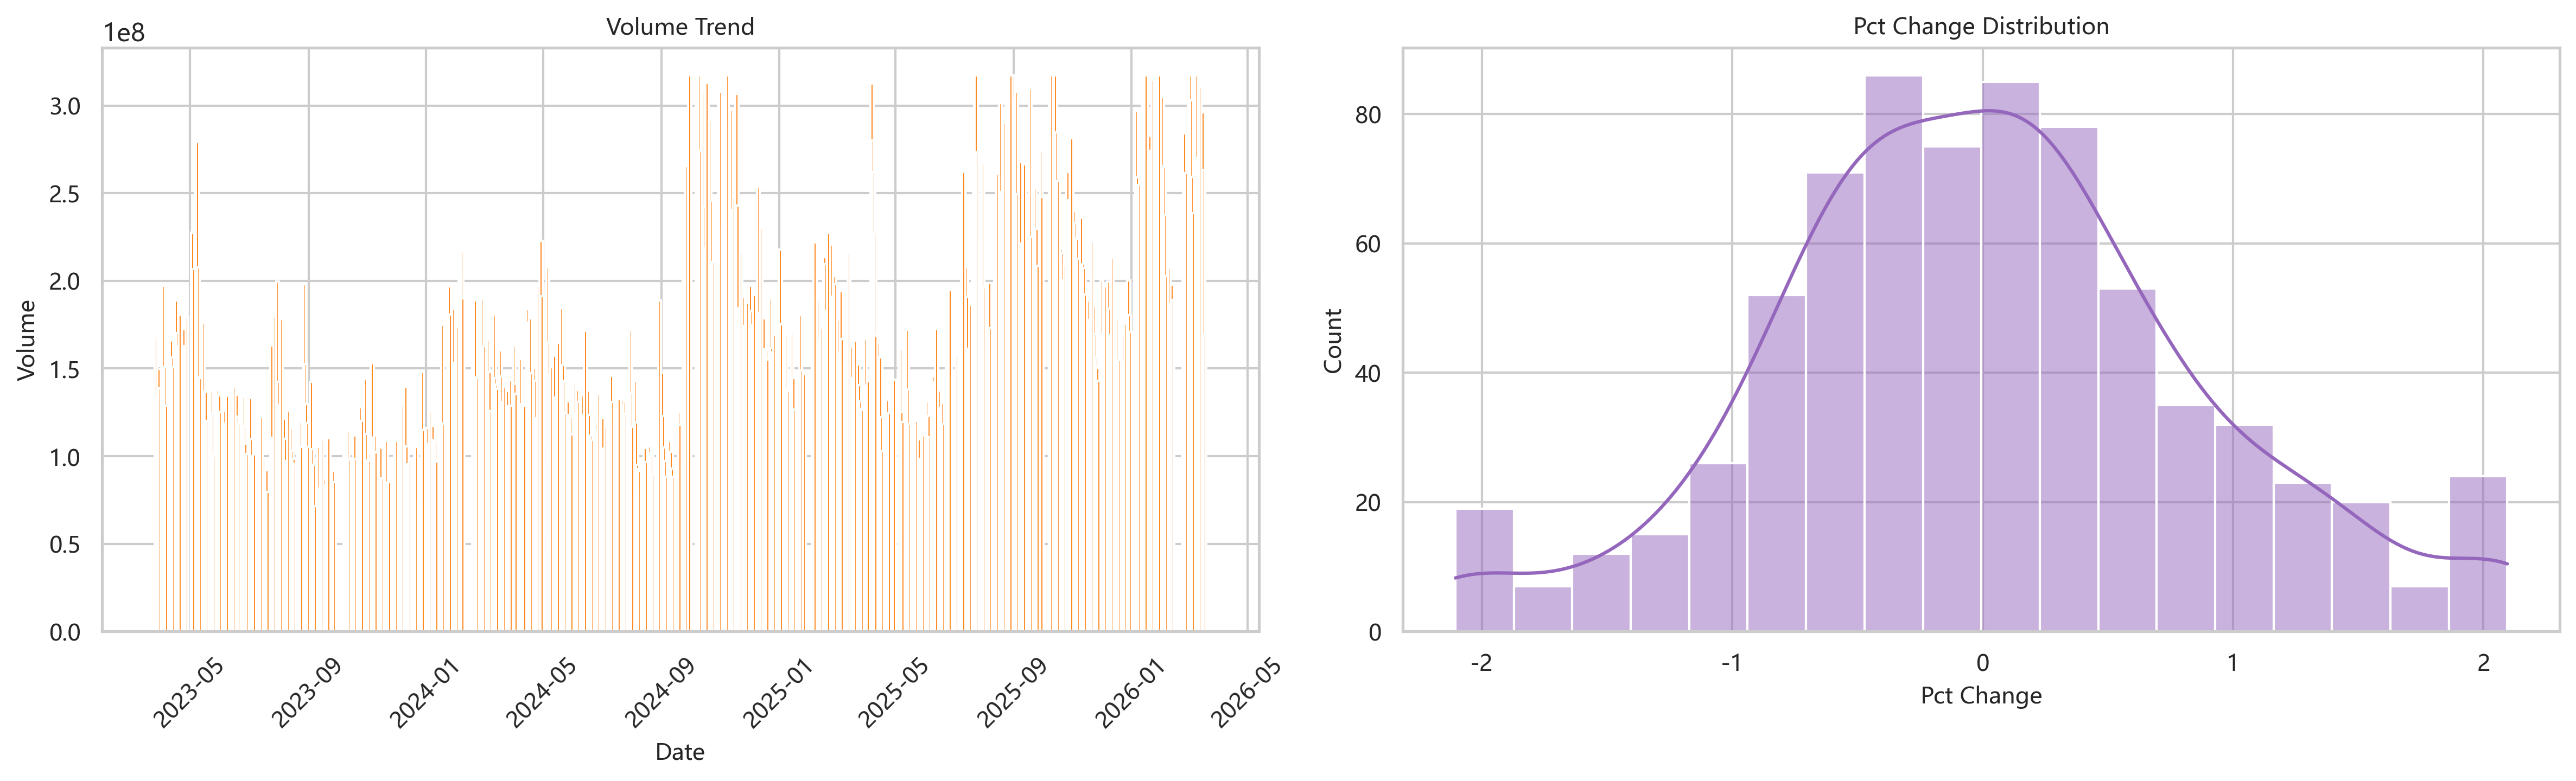
\includegraphics[width=0.88\textwidth]{../result/fig2_volume_pct.png}
\caption{交易量趋势与涨跌幅分布}
\end{figure}

该图进一步反映了市场交易行为特征。左侧交易量趋势图说明，不同阶段的市场活跃度差异明显，某些时期交易量显著抬升，可能对应市场情绪波动或指数快速变化阶段。右侧涨跌幅分布图整体接近以 0 为中心的集中分布，这说明多数交易日的涨跌幅较小，只有少数交易日出现较大波动。因此，涨跌幅虽然包含短期变化信息，但它更适合描述日内或相邻交易日之间的波动，不一定适合作为稳定的回归输入变量。

\subsection*{2.特征选择（包含：计算特征间相关系数，剔除高度相关冗余特征；剔除单一取值占比过高的无效特征；保留与目标变量相关性较强、有实际意义的特征）}
特征选择阶段首先计算候选特征之间以及各特征与目标变量之间的相关系数，并结合图形结果进行判断。实验中设置如下筛选原则：若两个特征之间的相关系数过高，则优先保留信息量更强、且更能体现时间依赖关系的特征；若某个特征单一取值占比过高，则认为信息量不足；若与目标变量相关性过弱，则剔除；若该特征由目标变量直接推导而来，则为避免目标泄漏不纳入最终建模。

通过筛选可知，开盘价、最高价、最低价以及多种滞后收盘价、滚动均值特征都与收盘价具有很强相关性，但它们之间也存在明显共线性，因此不能全部保留，否则会导致特征冗余和模型不稳定。为了让模型既利用当前市场状态，也保留一定的时间序列信息，实验在高相关成组特征中优先保留历史型特征。最终保留下来的特征为：交易量、年份、价格振幅、前 1 日收盘价（lag\_close\_1）和前 1 日成交量（lag\_volume\_1）。其中，涨跌幅因为由收盘价直接推导得到，属于潜在目标泄漏特征，因此被剔除；月份、日、星期、成交量变化率等特征由于与目标变量相关性较弱，也未进入最终模型。

\begin{figure}[H]
\centering
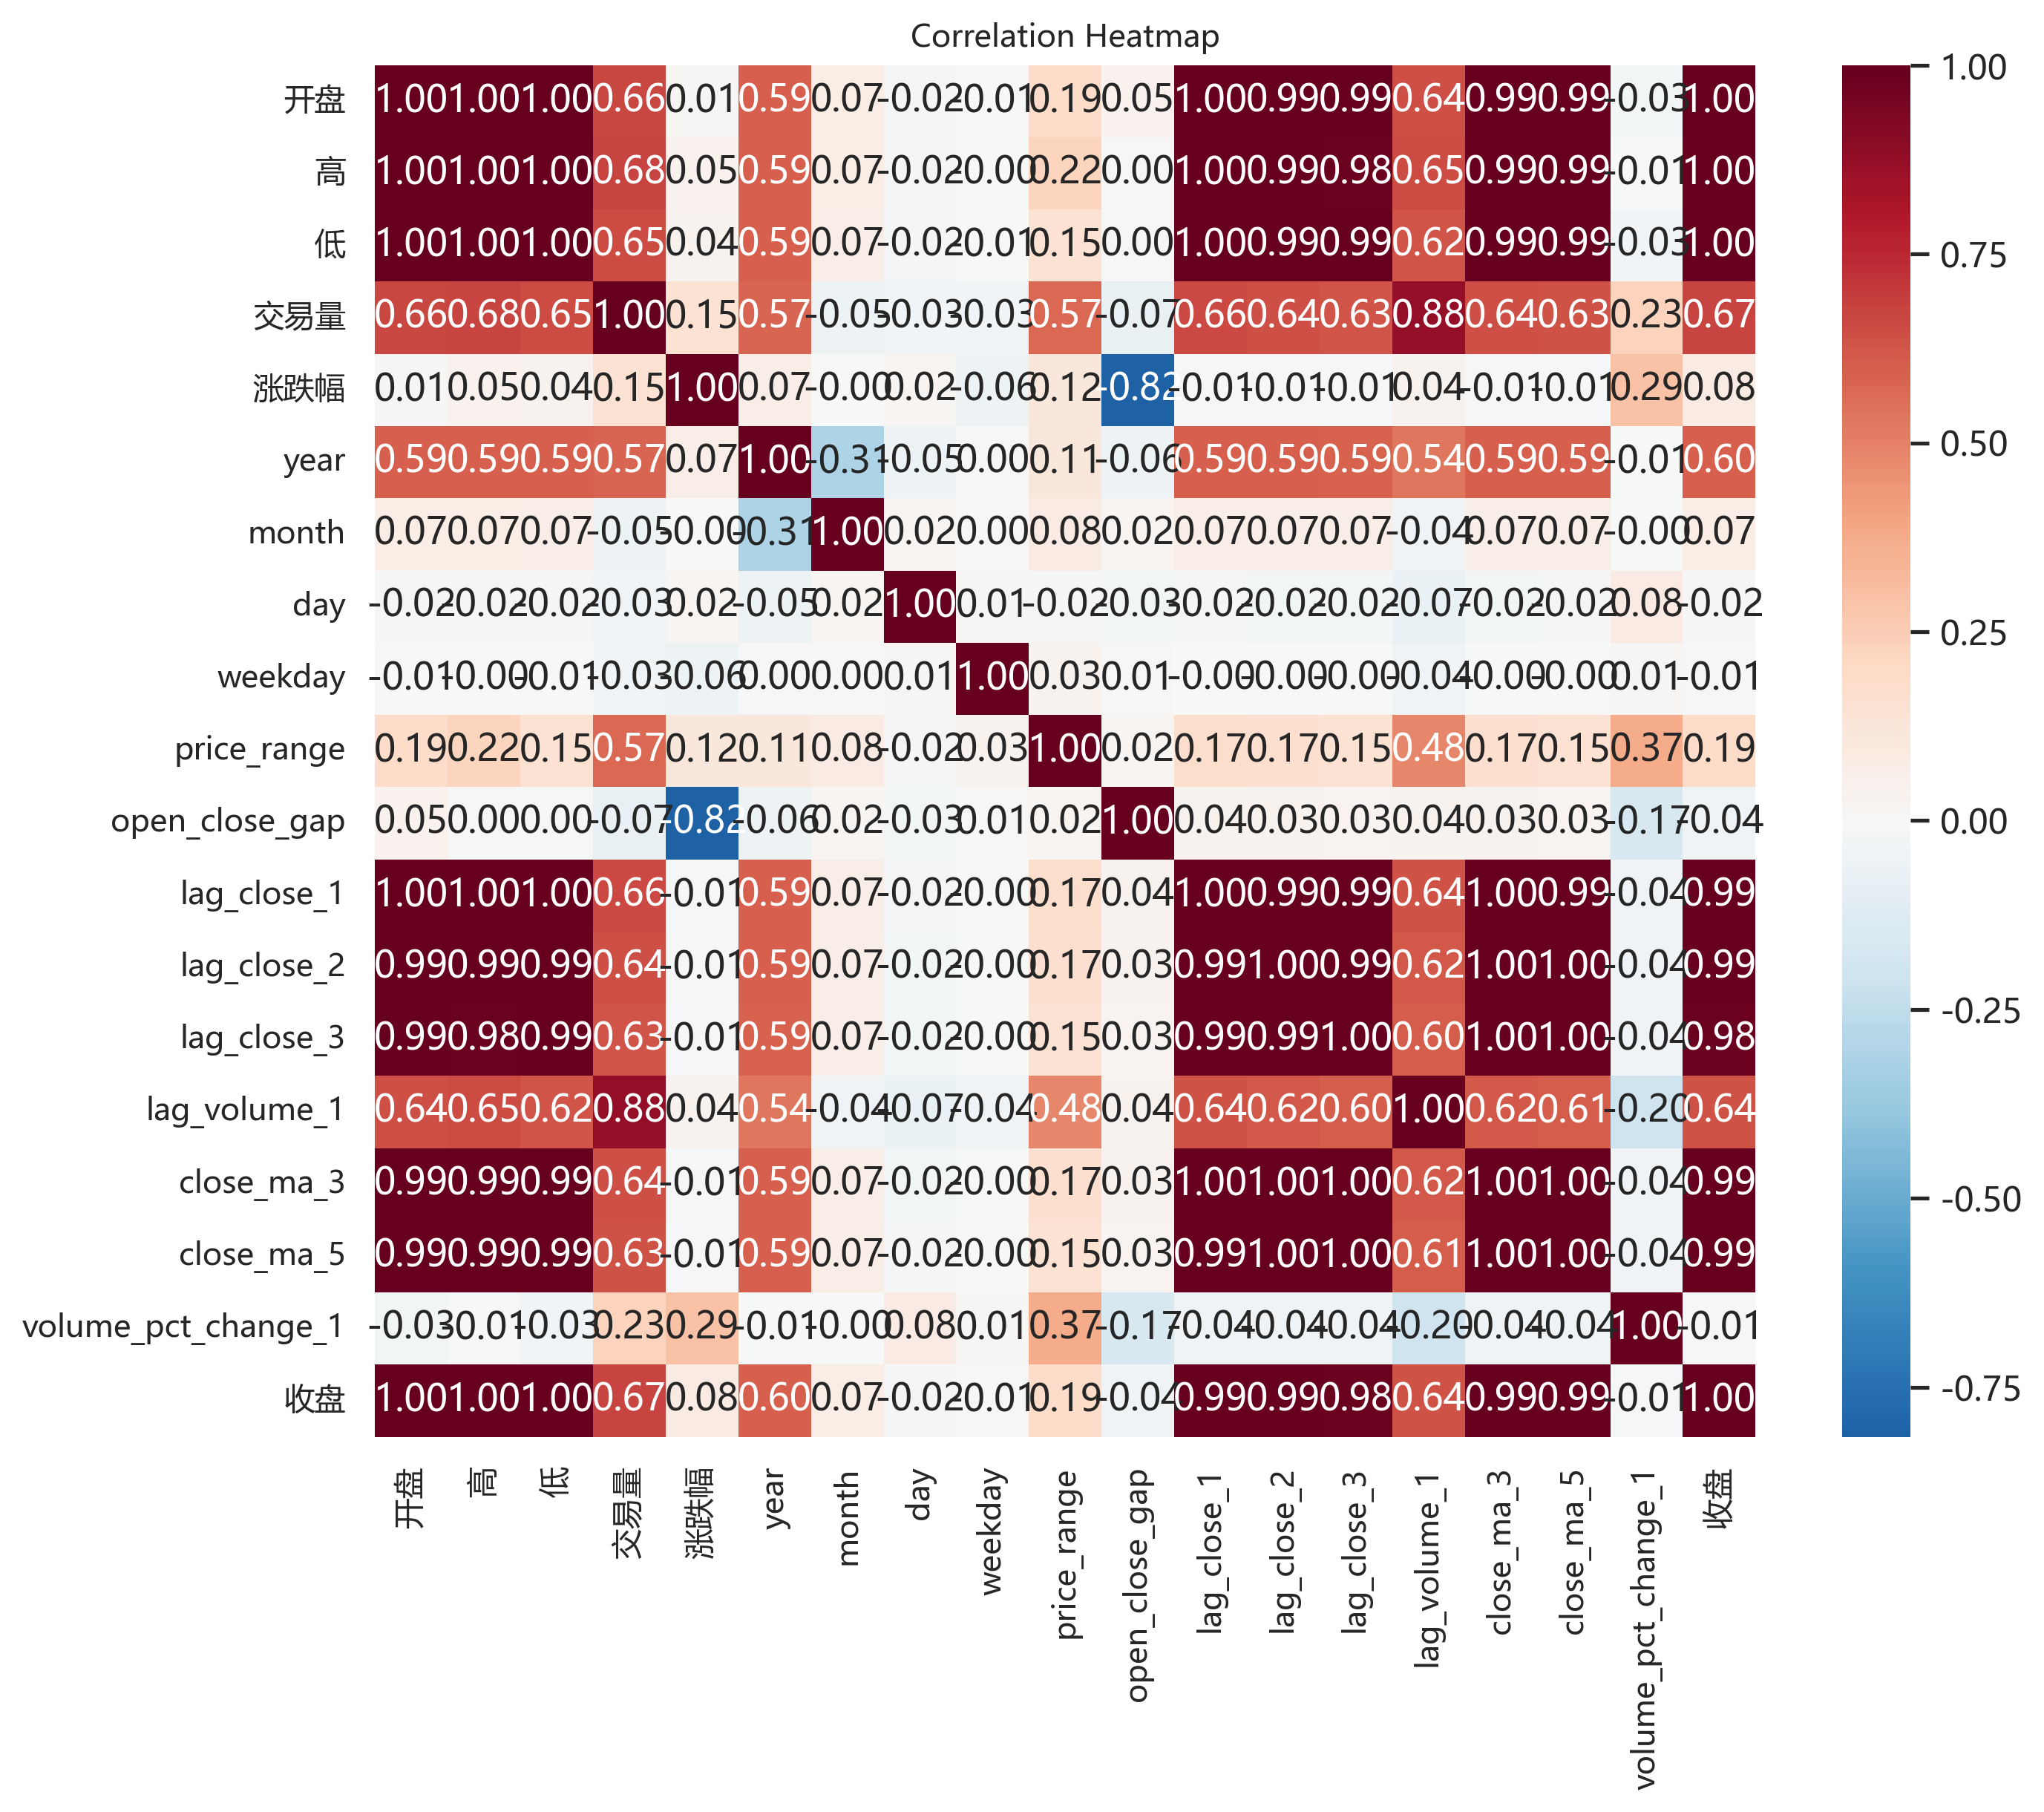
\includegraphics[width=0.82\textwidth]{../result/fig3_correlation_heatmap.png}
\caption{候选特征与目标变量的相关性热力图}
\end{figure}

从热力图可以直观看出，“高”“低”“开盘”与“收盘”之间的相关系数都接近 1，其中“高”与“收盘”的相关性最高，达到极强正相关水平。这说明最高价对解释收盘价变化具有最直接的作用。相比之下，交易量与收盘价存在中等程度相关，年份与收盘价也存在一定正相关，而月份、日、星期和涨跌幅与收盘价的相关性明显较弱。因此，热力图为后续保留“高、交易量、年份”提供了直接依据。

\begin{figure}[H]
\centering
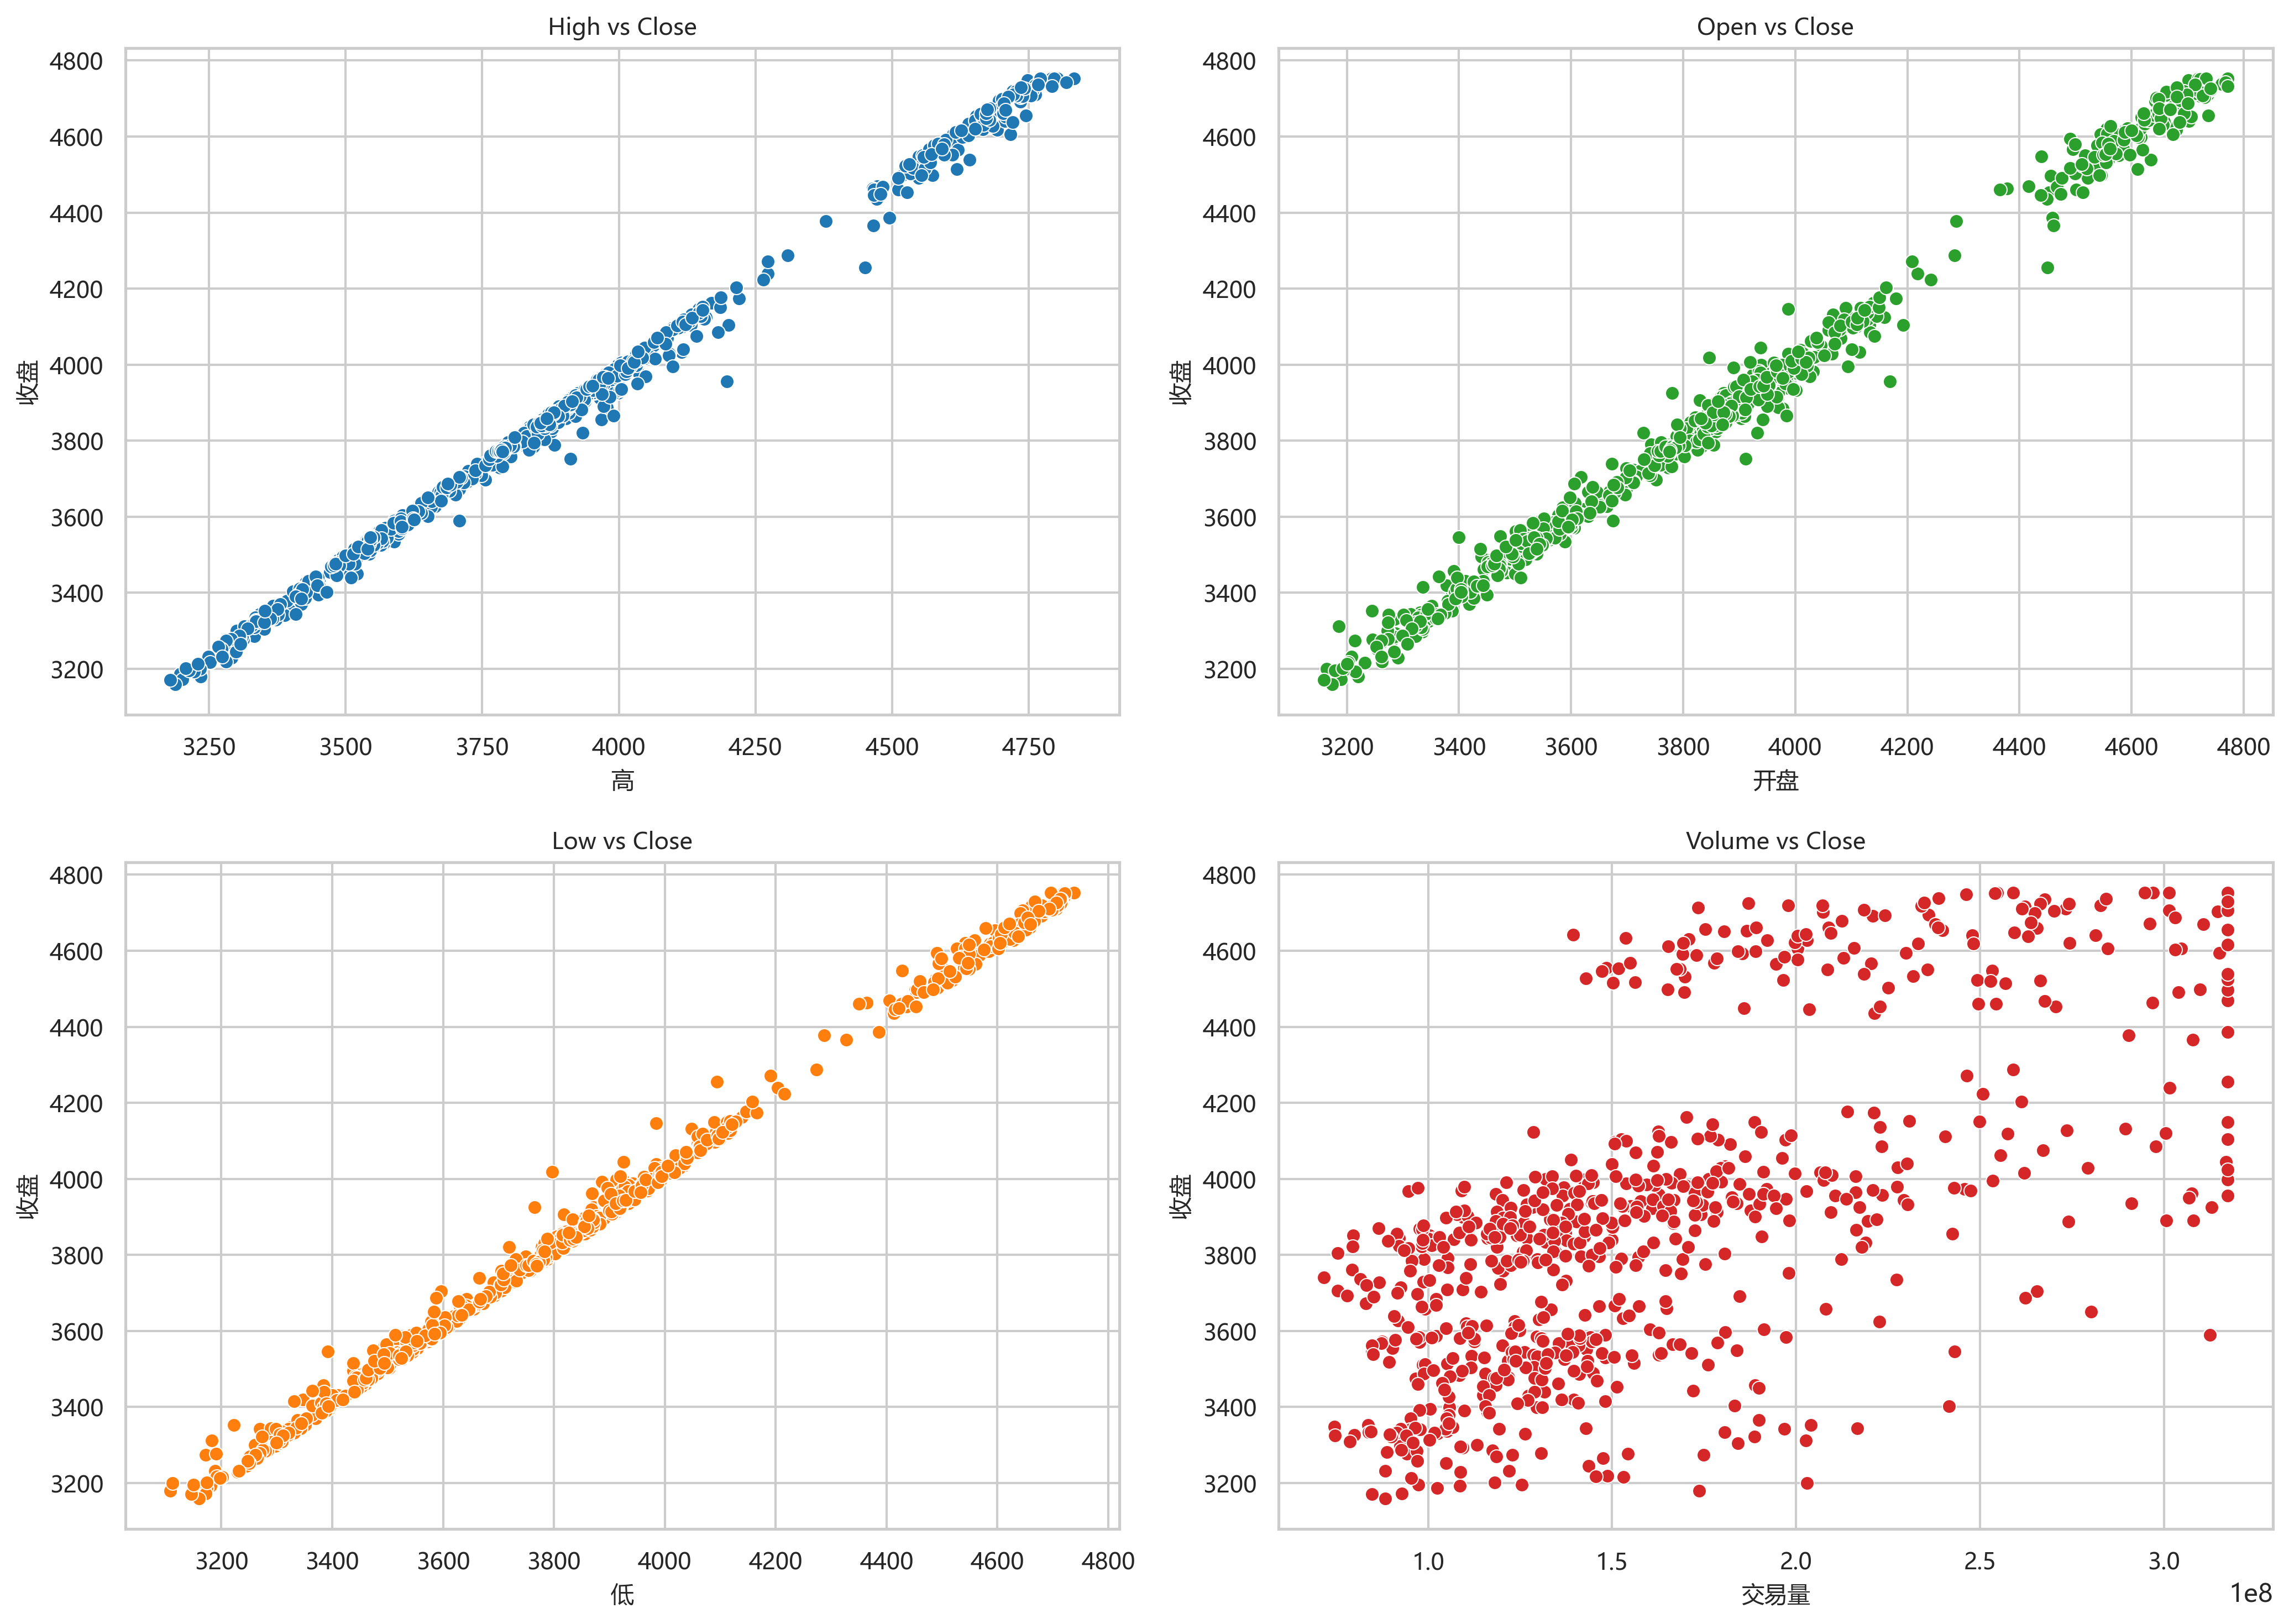
\includegraphics[width=0.92\textwidth]{../result/fig4_feature_scatter.png}
\caption{主要候选特征与收盘价的散点关系}
\end{figure}

散点图进一步验证了热力图结论。最高价、开盘价、最低价与收盘价之间都呈现明显的线性带状结构，说明价格类变量本身具有很强解释能力；交易量与收盘价的散点分布相对更分散，说明其解释能力弱于价格类特征，但仍具备一定辅助信息。结合新增的滞后收盘价和滚动均值特征的相关系数分析，可以判断最终保留特征在保证解释能力的同时，也引入了历史信息，从而使模型不再只依赖同一天的价格变量。

\subsection*{3. 数据集划分（包含：将数据划分为训练集与测试集，常用比例，训练集 70\%—80\%，测试集 20\%—30\%）}
由于本实验数据具有明显的时间顺序，如果采用随机划分方式，会破坏前后日期之间的真实关系，使测试结果不能真实反映模型对未来样本的预测能力。因此，本实验采用按时间顺序划分数据集的方法：前 80\% 样本作为训练集，后 20\% 样本作为测试集。这一比例符合常用的“训练集 70\%—80\%，测试集 20\%—30\%”原则。同时，滞后特征和滚动均值特征只使用历史信息构造，因此不会引入未来数据泄漏。

本次划分结果如下：训练集样本数为 576，测试集样本数为 144；训练集时间范围为 2023-03-27 至 2025-08-08，测试集时间范围为 2025-08-11 至 2026-03-18。这样的划分方式更贴近实际应用场景，即利用过去的数据训练模型，再对后续时间段的数据进行预测。

\subsection*{4. 构建与训练线性回归模型}
在特征筛选完成之后，以“交易量、年份、价格振幅、前 1 日收盘价、前 1 日成交量”作为输入特征，以“收盘价”作为目标变量，构建多元线性回归模型。模型形式如下：
\[
y=\beta_0+\beta_1x_1+\beta_2x_2+\beta_3x_3+\beta_4x_4+\beta_5x_5
\]
其中，$y$ 为收盘价，$x_1$、$x_2$、$x_3$、$x_4$、$x_5$ 分别表示交易量、年份、价格振幅、前 1 日收盘价和前 1 日成交量。

模型训练后得到的主要参数为：截距 $-487.2993$，交易量系数约为 $0$，年份系数 $0.2703$，价格振幅系数 $0.1098$，前 1 日收盘价系数 $0.9771$，前 1 日成交量系数约为 $0$。从系数大小来看，前 1 日收盘价对当前收盘价的影响最直接，说明历史价格水平是最重要的解释来源；价格振幅和年份提供了补充解释，而成交量相关特征更多体现辅助作用。

\begin{figure}[H]
\centering
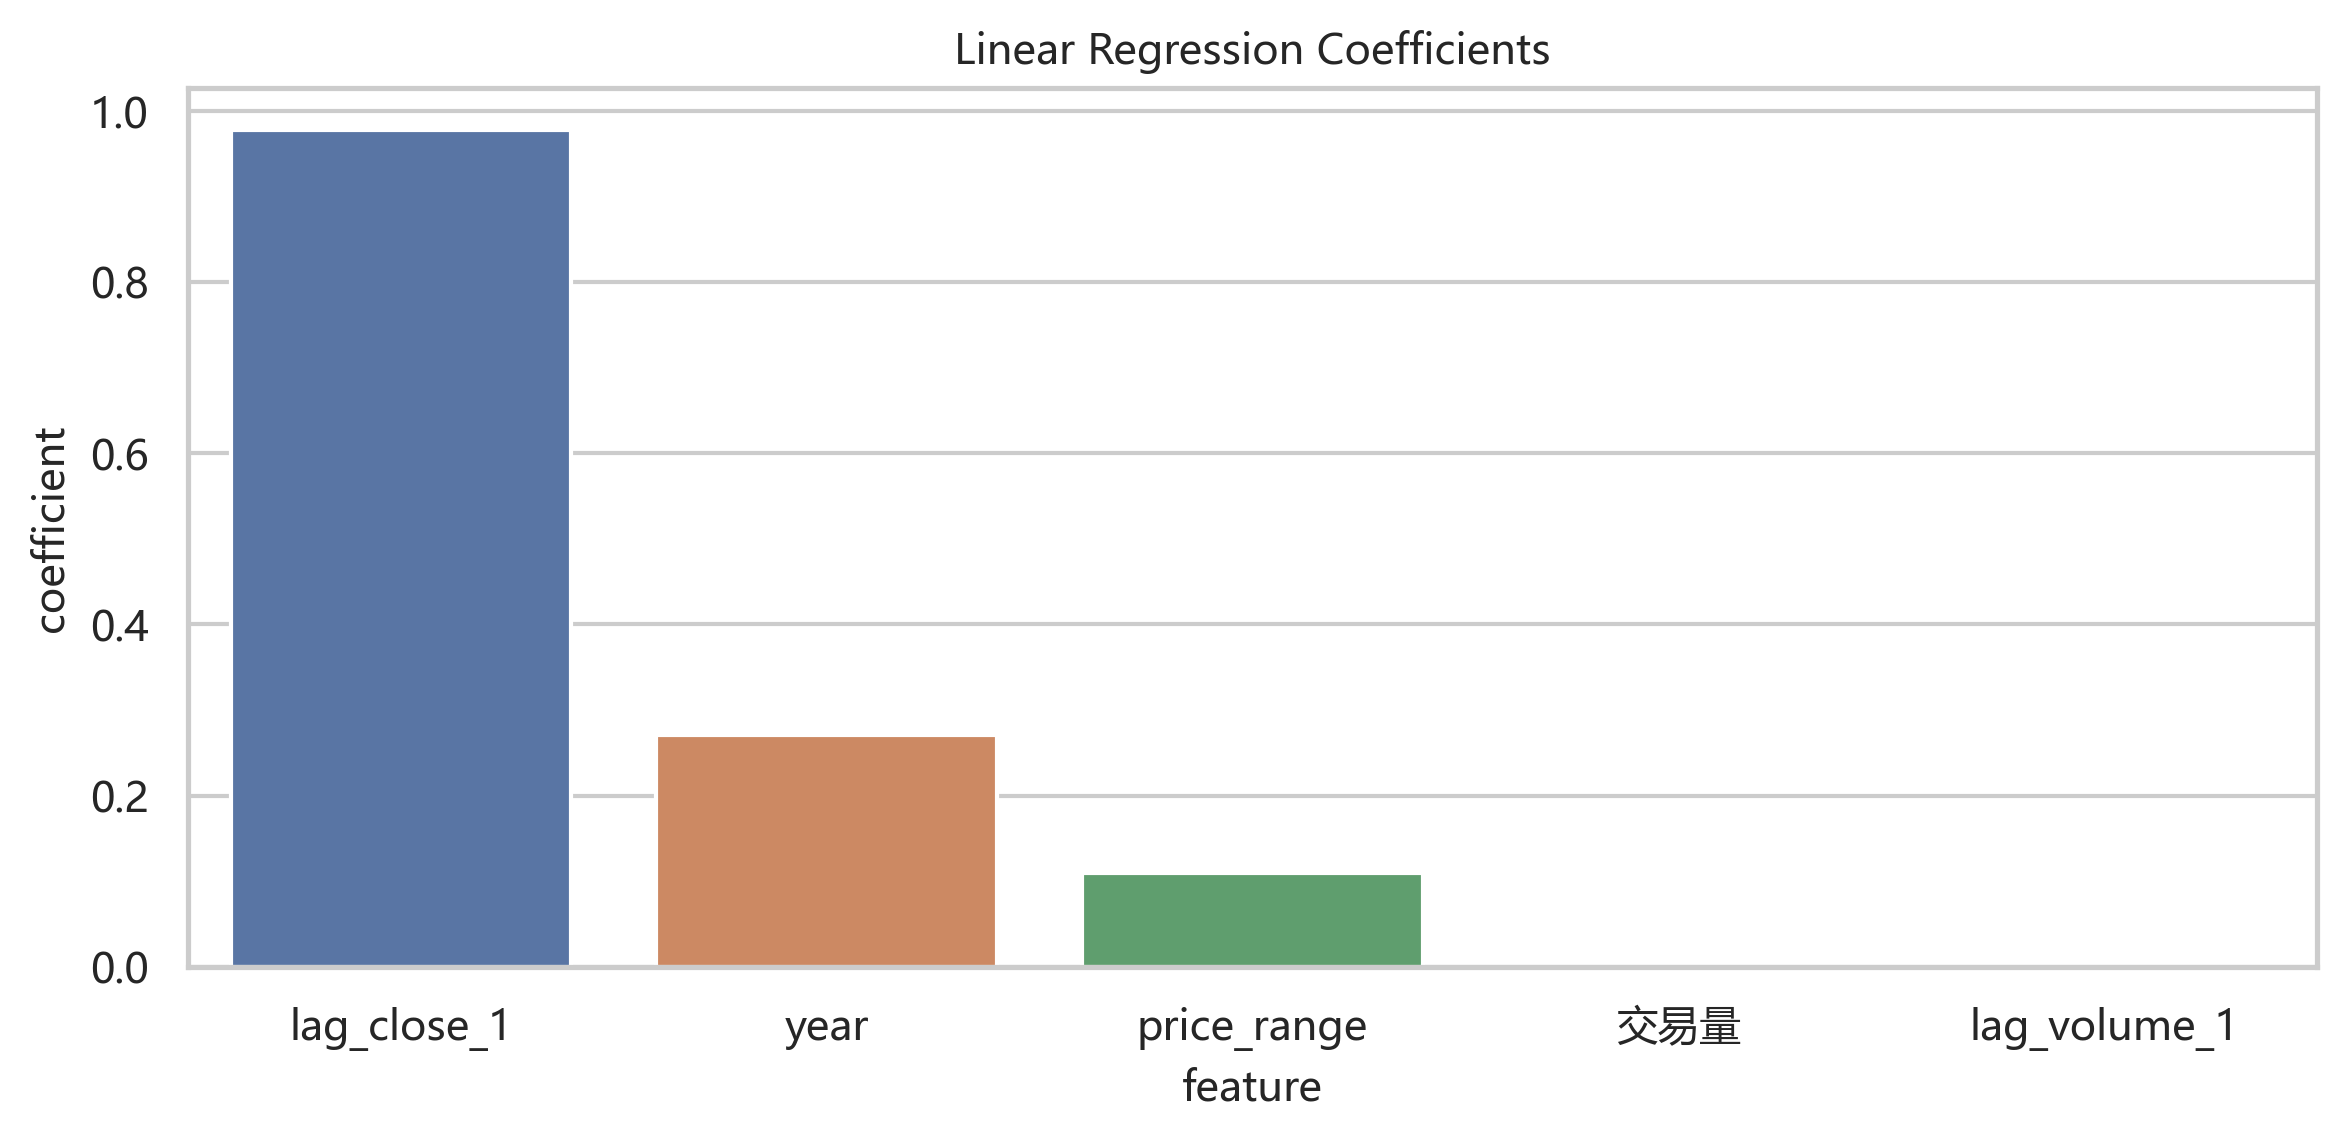
\includegraphics[width=0.68\textwidth]{../result/fig5_model_coefficients.png}
\caption{线性回归模型系数图}
\end{figure}

从系数图可以看出，绝对值最大的系数对应“前 1 日收盘价”，说明历史价格信息在最终模型中是最重要的解释变量。年份系数为正，说明随着年份推进，指数整体水平存在一定抬升趋势；价格振幅系数也具有一定影响，表明日内波动范围能够补充解释收盘价变化。交易量和前 1 日成交量的系数数值相对较小，说明它们对模型预测的直接线性贡献有限，但仍能为模型提供市场活跃度方面的辅助信息。整体来看，模型参数与前面的特征工程和特征筛选结果是一致的。

\subsection*{5. 模型预测与评估（用训练好的模型对测试集进行预测，可使用决定系数R²评估模型效果，R² 越接近 1 表示拟合越好）}
模型训练完成后，利用训练好的线性回归模型对测试集进行预测，并使用训练集 $R^2$、测试集 $R^2$、平均绝对误差 MAE 和均方根误差 RMSE 进行综合评估。其中，$R^2$ 越接近 1，表示模型对目标变量的解释能力越强，拟合效果越好。

实验得到的评价结果如下：
\begin{table}[H]
\centering
\begin{tabular}{cc}
\toprule
指标 & 数值 \\
\midrule
训练集 $R^2$ & 0.9755 \\
测试集 $R^2$ & 0.8912 \\
MAE & 35.4496 \\
RMSE & 44.5635 \\
\bottomrule
\end{tabular}
\end{table}

从结果可以看出，训练集 $R^2$ 为 0.9755，测试集 $R^2$ 为 0.8912，说明模型在训练集上拟合较好，在测试集上仍保持了较强的解释能力，但相比只依赖当日价格变量的模型，加入历史特征后模型表现更接近真实的时序预测场景。MAE 为 35.4496，表示模型预测的平均绝对误差约为 35.45 点；RMSE 为 44.5635，说明部分波动较大的交易日会带来更明显的预测偏差。综合这些指标，可以认为本模型在保留可解释性的同时，也较好体现了时间依赖特征对收盘价预测的作用。

\begin{figure}[H]
\centering
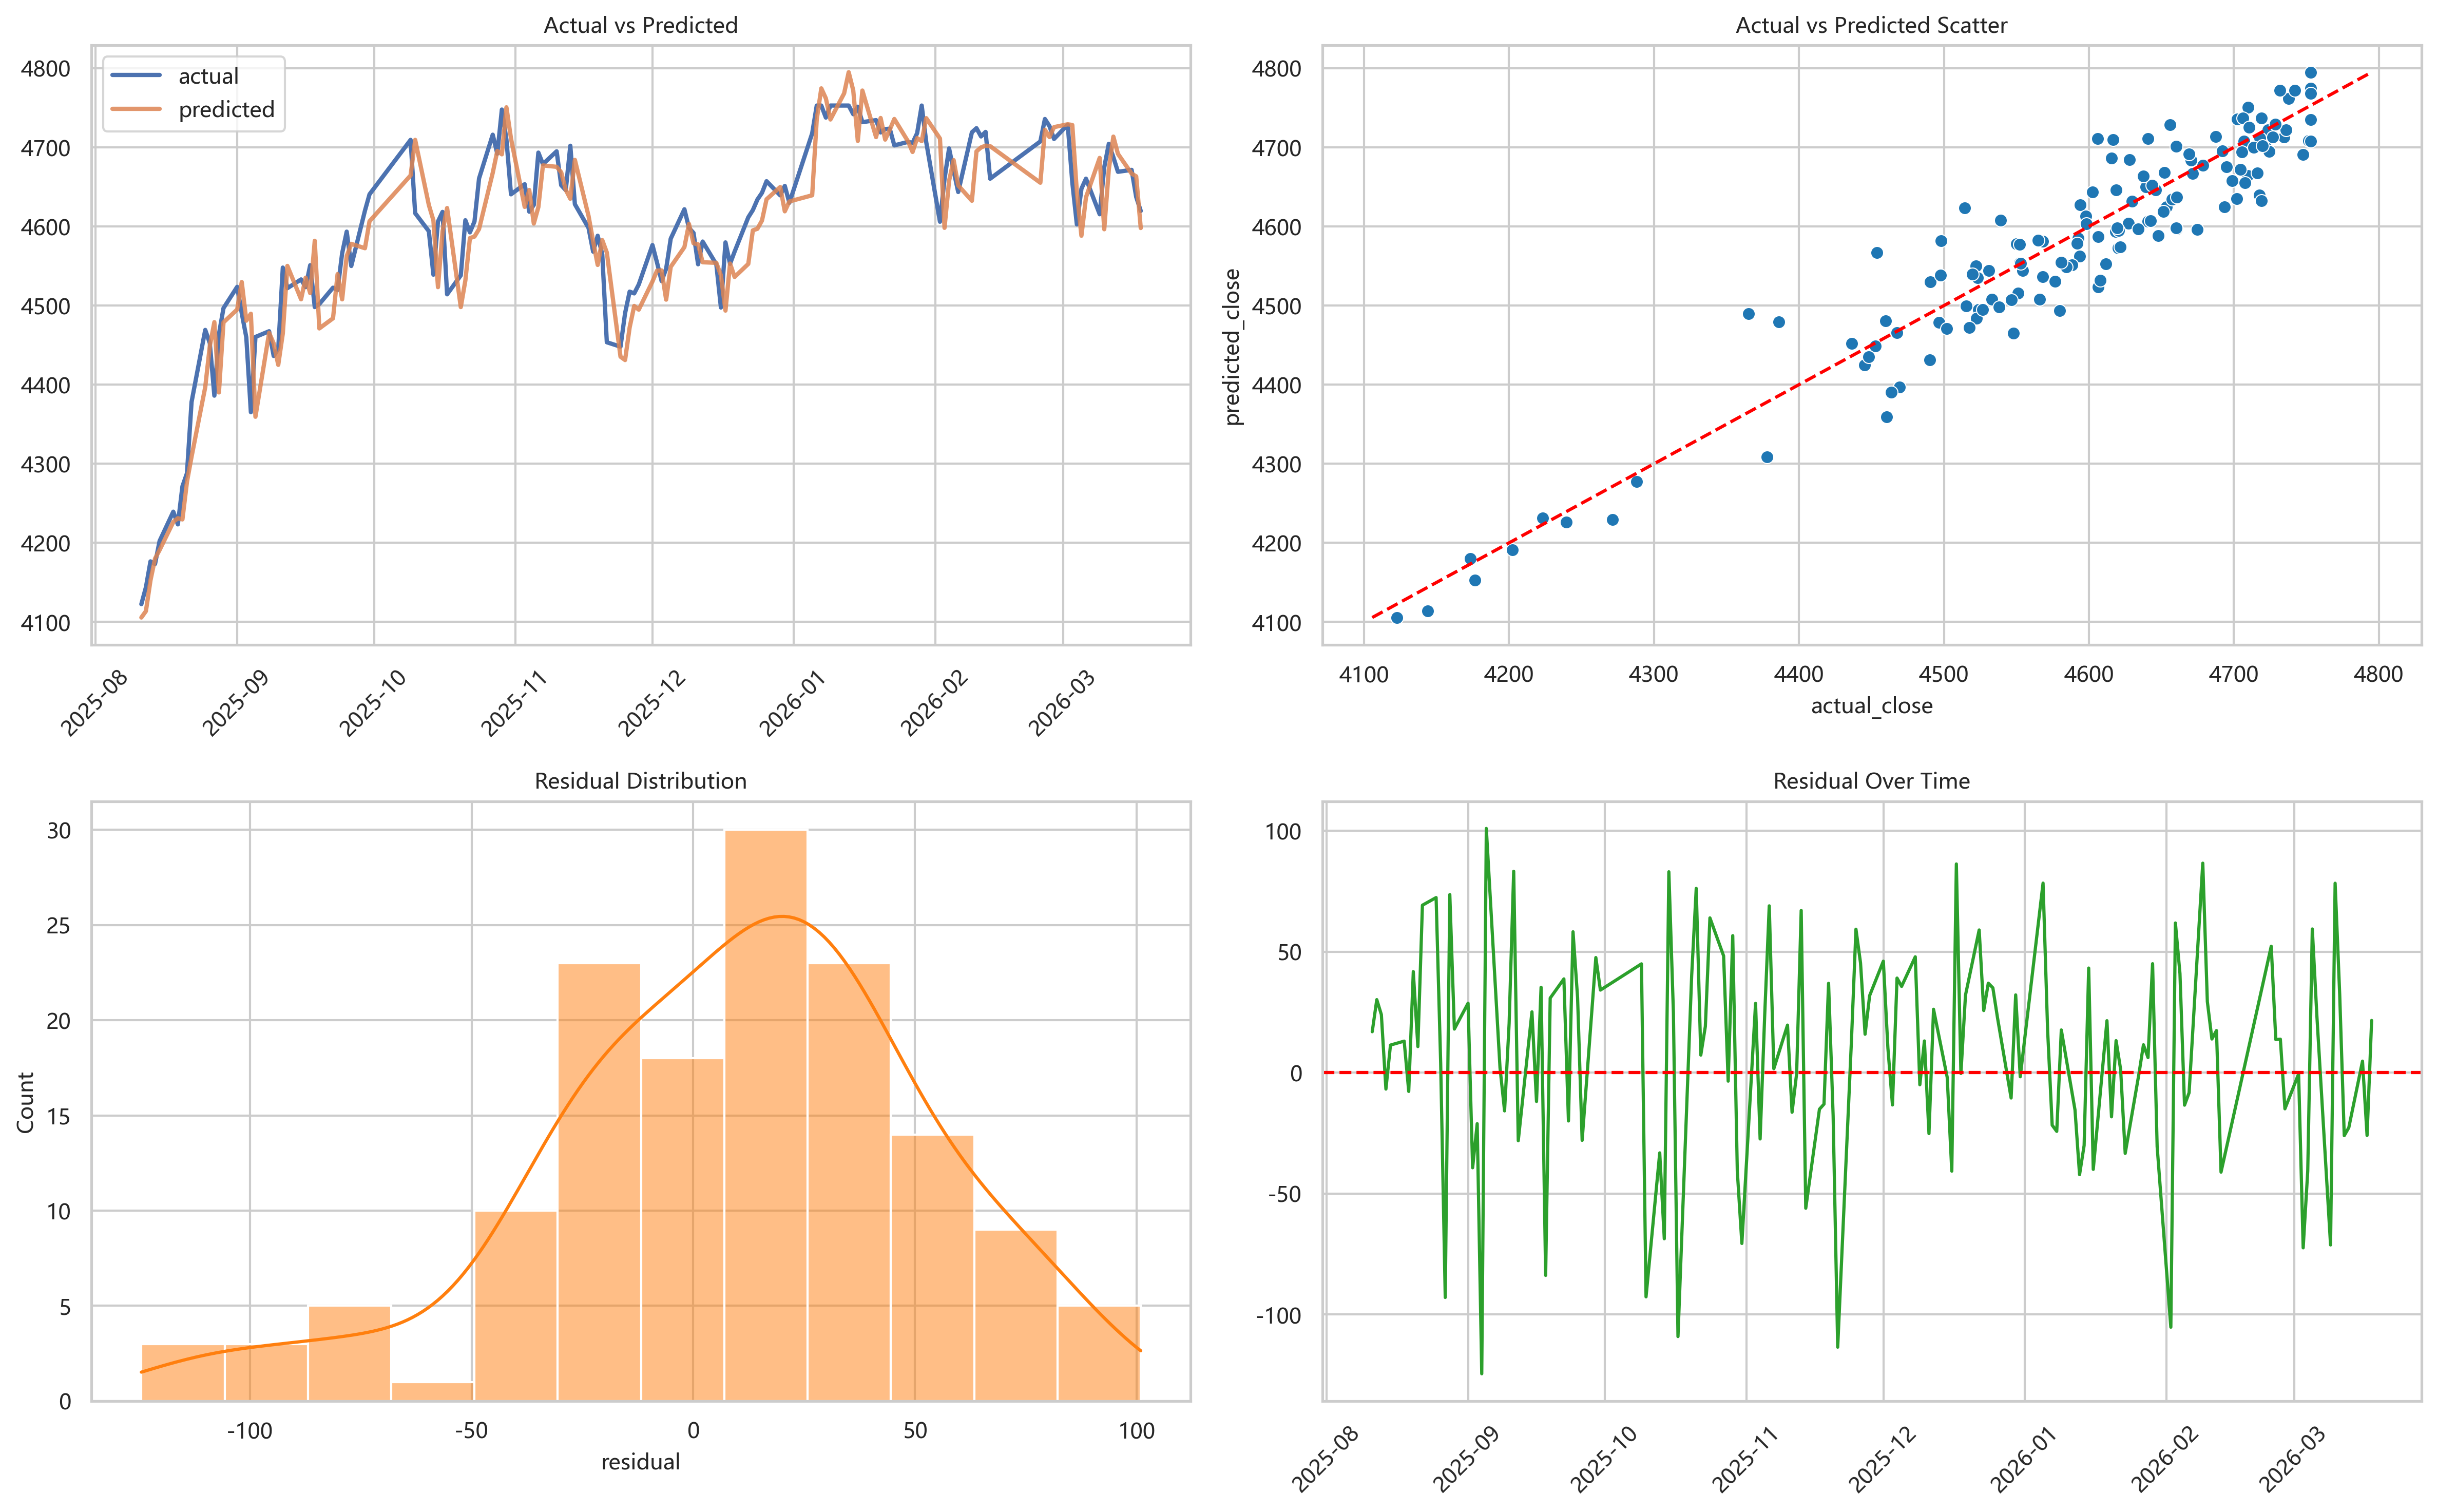
\includegraphics[width=0.92\textwidth]{../result/fig6_prediction_residuals.png}
\caption{测试集真实值、预测值及残差分析}
\end{figure}

该图从多个角度展示了模型预测效果。左上角真实值与预测值对比图中，两条曲线整体变化趋势基本一致，说明模型能够较好地跟随收盘价波动。右上角真实值与预测值散点图中，样本点大多分布在对角线附近，说明预测值与真实值较接近。左下角残差分布图显示，残差主要集中在 0 附近，说明模型整体没有明显系统性偏差。右下角残差随时间变化图中，大部分残差在 0 附近波动，只有少数时段出现较大偏离，说明模型在多数测试样本上的预测较稳定。

\subsection*{6.其他，可选做}
除完成题目要求的基本流程外，本实验还补充了较为完整的可视化分析。通过缺失值统计图、分布图、箱线图、趋势图、热力图、散点图、系数图和残差图，不仅能够更直观地观察数据分布和模型表现，也便于从图像角度解释为什么保留某些特征、为什么模型能够取得较高的 $R^2$ 分数。这些补充内容有助于提高实验报告的完整性和说服力。

\section*{五、实验结果与分析（保留的特征列表及选择理由，描述训练集和测试集样本数量，训练集与测试集的 R²分数，对模型效果进行评价）}
本实验最终保留的特征列表为：\textbf{交易量、年份、价格振幅、前 1 日收盘价、前 1 日成交量}。

其选择理由可以总结如下：
\begin{enumerate}[label=（\arabic*）]
\item 前 1 日收盘价与当前收盘价保持极强相关性，且能够体现时间依赖结构，因此是最关键的历史特征；
\item 交易量和前 1 日成交量可以共同反映市场活跃程度，为价格预测提供辅助信息；
\item 年份体现了不同年度市场整体水平的差异，价格振幅能够反映日内波动范围，因此二者一并保留；
\item 开盘价、最高价、最低价以及多种滚动均值特征虽然也与收盘价高度相关，但它们之间共线性明显，因此只保留更能体现历史信息的代表性特征；
\item 涨跌幅由收盘价直接推导得到，若保留会引入目标泄漏，影响模型评价的客观性，因此剔除；
\item 月份、日、星期、成交量变化率等特征与目标变量相关性较弱，对模型贡献有限，因此未纳入最终建模。
\end{enumerate}

在数据集划分方面，训练集样本数为 576，测试集样本数为 144。由于采用了按时间顺序划分的方式，因此测试集更能反映模型对“未来时间段”样本的预测能力，而不仅仅是对随机样本的拟合能力。

从模型分数来看，训练集 $R^2=0.9755$，测试集 $R^2=0.8912$。二者都保持在较高水平，说明模型对收盘价仍具有较强解释能力；同时训练集与测试集之间存在一定差距，这也说明在引入更符合实际预测逻辑的历史特征后，模型评估结果更加客观，不再过度依赖同一天价格变量所带来的“近似同步拟合”效果。对于一个仅使用 5 个特征的线性回归模型而言，这样的结果仍然说明所保留特征具有较高有效性。

进一步结合误差指标分析，MAE 为 35.4496，说明模型在测试集上的平均绝对偏差约为 35 个指数点；RMSE 为 44.5635，略高于 MAE，说明少数样本存在相对较大的误差，但整体误差水平仍处于可接受范围。将这些指标与真实值和预测值对比图、残差分布图结合起来看，可以发现模型在大多数日期上仍能够较好地跟踪指数变化趋势，只是在局部波动较剧烈的时段预测偏差会稍大一些。

从特征作用的角度看，前 1 日收盘价几乎决定了模型的主要拟合能力，这说明历史价格水平对下一交易日收盘价具有显著解释作用；价格振幅则补充了日内波动信息；交易量与前 1 日成交量共同补充了市场活跃度信息；年份用于刻画指数所处的阶段性水平。因此，最终模型虽然形式简单，但相比只依赖当日价格变量的方案，更符合时间序列预测的基本思路，也具有更好的解释性。

当然，也需要客观看待模型的局限性。本实验数据本质上属于时间序列数据，虽然已经引入了滞后特征和滑动窗口统计量，但线性回归模型本身仍主要刻画线性关系，难以充分捕捉更复杂的非线性时序模式。因此，该模型更适合作为课程实验中的基础回归案例，用于说明特征选择、数据清洗、时序特征构造、线性建模和模型评估的完整流程；如果用于更复杂的真实金融预测场景，还可以进一步尝试岭回归、树模型，或者更适合时序问题的模型进行对比。

总体来看，本实验最终保留的特征合理，训练集与测试集划分规范，模型评估指标良好，说明本次上机实验较好地完成了题目要求，并达到了预期分析目的。

\section*{六、实验总结}
本次实验围绕“特征选择、数据集划分与线性回归”展开，完整实现了数据读取、数据预处理、特征筛选、训练集与测试集划分、模型训练以及模型评估的全过程。通过实验，我不仅掌握了如何从原始数据中清洗无效信息、剔除冗余特征，也进一步理解了特征选择对于模型性能和模型解释性的影响。

从实验结果来看，所建立的线性回归模型在测试集上的 $R^2$ 为 0.8912，说明模型整体拟合效果较好，能够较准确地描述收盘价与关键特征之间的关系。同时，本实验也让我认识到，在处理金融类数据时，不仅要关注模型的数值指标，还要结合数据来源、特征意义、时间顺序以及目标泄漏等问题进行综合判断。

总体而言，本次实验顺利完成了课程要求，也为后续进一步学习更复杂的回归模型和时间序列预测方法打下了基础。

\end{document}
